\section{Axes d'améliorations}

\subsection{Suggestion modèle de prédiction}

\subsubsection{GPU}

Comme il a été mentionné précédemment, on utilise une \textbf{Nvidia L40 S}.
Même avec cette configuration, on est limité en ce qui concerne la \textbf{batch\_size} de notre modèle. 
La taille du lot (batch size) est un hyperparamètre qui détermine le nombre d'échantillons à traiter avant de mettre à jour les poids du modèle.
Pour l'augmenter, il faudrait utiliser plusieurs GPU et faire probablement de l'entrainement distribué pour permette de traiter plusieurs lots et potentiellement améliorer le modèle.

\textbf{NB :} Si il le GPU n'est pas assez puissant lors de l'exéction du modèle, il serai possible que des erreurs liés à la mémoire apparaissent. Souvent des erreurs de type \texttt{CUDA out of memory} apparaissent.

\subsubsection{Hyperparamètres}
Pour ce projet, on a utilisé un algorithme d'optimisation des hyperparamètres (ex : batch\_size) via la librairie \texttt{hyperopt}.
Cependant, on a été limité en termes de temps ce qui a valu une dimunution de l'espace de recherche de ces hyperparamètres.  
À l'avenir il serait utile d'agrandir l'espace de recherche des hyperparamètres avec des valeurs plus grandes dans l'espace de recherche pour étendre la recherche des meilleures hyperparamètres.

\begin{figure}[H]
    \centering
    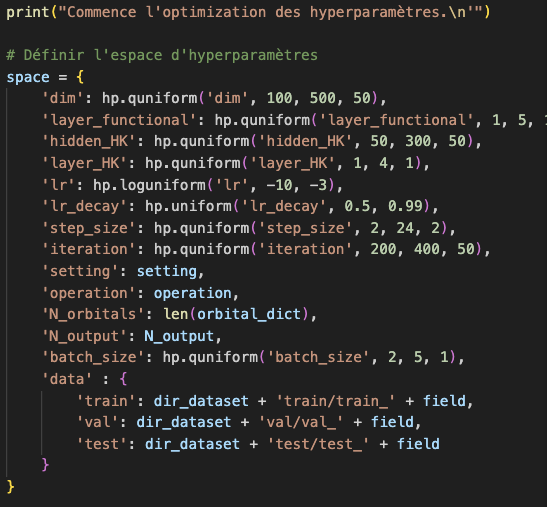
\includegraphics[width=0.6\textwidth]{Overview/hyper.png}
    \caption{Espace de recherche des Hyperparamètres}
\end{figure}

\subsubsection{Fonction de pertes du modèle et fontion d'activation}
La fonction de perte est un élément clé dans l'entraînement d'un modèle d'apprentissage automatique.
Elle mesure la différence entre les prédictions du modèle et les valeurs réelles.
Dans le cas de la prédiction de PCE, la fonction de perte utilisée est la \textbf{MAE} (Mean Absolute Error).
Le MAE est une mesure linéaire de la différence entre les valeurs prédites et les valeurs réelles.
Pour espérer mieux extrapoler les données, il serait intéressant d'utiliser une fonction de perte non linéaire comme la \textbf{Huber Loss ou RMSE} qui est moins sensible aux valeurs aberrantes que la MAE.

Pour les fonctions d'activation, il serait utile de les changer pour vérifier l'effet l'obtenu sur la prédiction.
Notamment, celle préente à la couche de sortie du DNN pour prédire de PCE, puisque le PCE doit être strictement positif on pourrait envisager uen fonction d'activation comme \textbf{ReLU} par exemple.

\subsection{Modèle de génération}

\subsubsection{Traduction SMILES en SELFIES}

L'une des principales difficultés rencontrées concerne la conversion des représentations SMILES en SELFIES (Self-Referencing Embedded Strings). Bien que SELFIES soit plus robuste pour la génération de structures valides, sa conversion depuis des SMILES complexes n’est pas toujours triviale. Certains encodages échouent ou génèrent des représentations ambiguës, nécessitant une étape supplémentaire de validation et de correction. Cela introduit une complexité additionnelle dans le pipeline de traitement et peut réduire la qualité des entrées pour le modèle génératif.

\subsubsection{Génération de molécules via NO-Operation (NOP)}

Lors de la génération de nouvelles structures moléculaires, nous avons observé que certains modèles avaient tendance à produire un grand nombre de caractères de type NO-Operation (NOP), c’est-à-dire des éléments neutres ou répétitifs sans signification chimique. Cela peut résulter d’un mauvais apprentissage des règles syntaxiques moléculaires ou d’un sur-apprentissage sur les motifs fréquents. La présence excessive de NOP réduit la diversité et la qualité des molécules générées, ce qui compromet leur validité et leur pertinence.
